\chapter{Generalisation and validation (introduction)}\label{ch-04}

The fourth lecture concludes the introduction to ML by addressing the
central theme of the course: \textbf{generalisation}. Through a
concrete example (polynomial fitting) we see the phenomena of
\textbf{underfitting} and \textbf{overfitting}, give a first
formalisation with \textbf{Statistical Learning Theory} and the
\textbf{VC-dimension}, and introduce the basic \textbf{validation}
techniques, accuracy measures for classification and the design cycle
of an ML system.

\section{ML in a nutshell}\label{il-ml-in-breve}

Let us recap the ingredients seen in the previous lectures:

\begin{itemize}
\tightlist
\item
  \textbf{Data}: the available experience, represented as vectors,
  structures, etc.
\item
  \textbf{Task}: supervised (classification, regression),
  unsupervised, \ldots{} For example, given labelled examples, find a
  good approximation of the unknown \(f\).
\item
  \textbf{Model}: describes the relationships among data and defines
  the class of functions the machine can implement (the hypothesis
  space).
\item
  \textbf{Learning algorithm}: given task and model, performs a
  (heuristic) search in the space of hypotheses valid on the data,
  fitting the free parameters of the model.
\item
  \textbf{Validation}: evaluates the generalisation capability of the
  hypothesis found.
\end{itemize}

The underlying message remains: \emph{easy use of ML tools} versus
\emph{correct and aware use of ML}.

\section{The fundamental problems of
ML}\label{i-problemi-fondamentali-del-ml}

\subsection{An ill-posed problem}\label{un-problema-mal-posto}

Inferring general functions from known data is an \textbf{ill-posed
problem}: in principle the solution is not unique, and with finite data
we cannot expect to find the exact solution. This is why we work with
a \textbf{restricted hypothesis space} (recall inductive bias). Two
questions guide the study of models:

\begin{itemize}
\tightlist
\item
  \textbf{What can we represent?} (if a function is not representable,
  it cannot be learned either);
\item
  \textbf{What can we learn?} (a secondary question with respect to
  the first).
\end{itemize}

\subsection{Generalisation and
overfitting}\label{generalizzazione-e-overfitting}

We distinguish the \textbf{learning phase}, in which the model is built
(including training), from the \textbf{prediction phase}, in which the
learned function is evaluated on new samples (generalisation
capability).

\begin{boxdefinition}{Inductive learning hypothesis}

\emph{Any hypothesis \(h\) that approximates \(f\) well on the training
examples will also approximate \(f\) well on new, unseen instances.}

\end{boxdefinition}

The question mark the professor puts next to this hypothesis is
intentional: \textbf{it is not always true}, and this is exactly where
overfitting arises.

\begin{boxdefinition}{Overfitting}

A learner \textbf{overfits} the data if it outputs a hypothesis
\(h \in H\) with true (generalisation, \emph{risk}) error \(R\) and
empirical (training) error \(E\), when there exists another
\(h' \in H\) with \[
E' > E \qquad \text{but} \qquad R' < R.
\] In other words, \(h'\) fits the training data \emph{worse} but is
\emph{better} on new data.

\end{boxdefinition}

The critical aspect thus becomes \textbf{accuracy estimation}, which
can be tackled \textbf{theoretically} (Statistical Learning Theory) or
\textbf{empirically} (training and test error, cross-validation
techniques).

\section{A case study: polynomial
fitting}\label{un-caso-di-studio-il-fitting-polinomiale}

To see concretely the role of model complexity we use a regression
example with a parametric model: the hypothesis space is the set of
\textbf{polynomials of degree \(M\)}, \[
h_\mathbf{w}(x) = w_0 + w_1 x + w_2 x^2 + \dots + w_M x^M = \sum_{j=0}^{M} w_j x^j.
\] The complexity of the hypothesis grows with the degree \(M\); \(l\)
is the number of examples.

\begin{boxwarning}{Artificial example}

It is a simplified and unrealistic task: a single input variable, and
we know the target function in advance. It only serves to visualise the
concepts.

\end{boxwarning}

The target function is \(\sin(2\pi x)\) with added \textbf{Gaussian
noise}: this is why the samples do not lie exactly on the ``true''
green curve.

\begin{figure}[htbp]
\centering
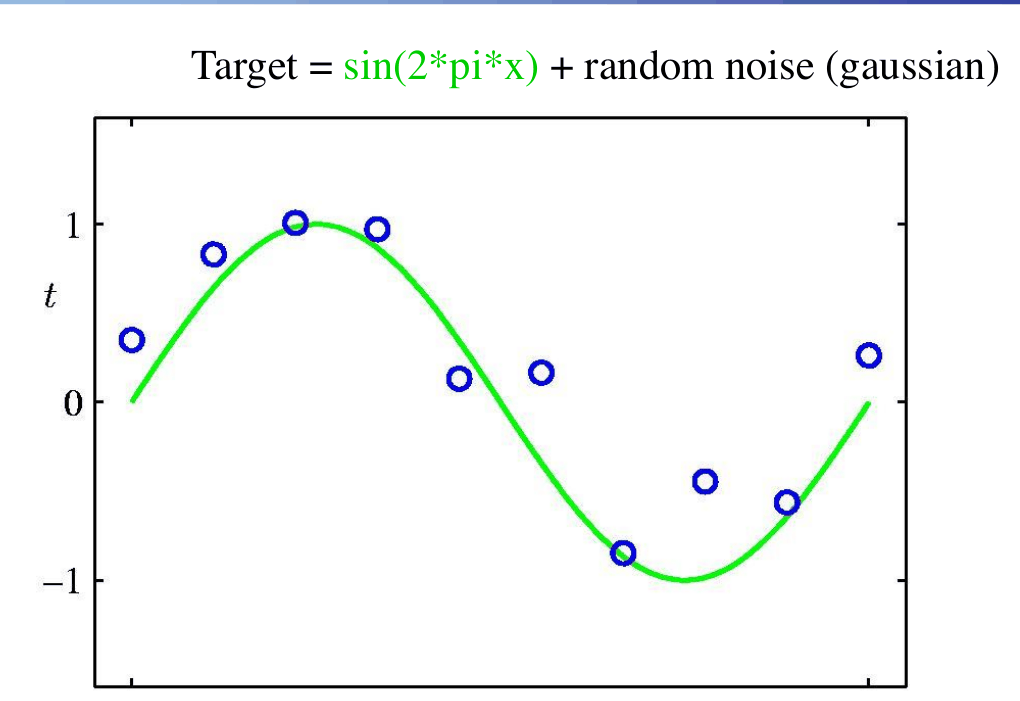
\includegraphics[width=0.54\linewidth,height=0.42\textheight,keepaspectratio]{images/04-l4_target-seno.png}
\caption{The target function \(\sin(2\pi x)\) (in green) and the noisy
training samples (in blue).}
\end{figure}

To find the best parameters, the \textbf{sum of squared errors} is
minimised: \[
E(\mathbf{w}) = \sum_{p=1}^{l} \big(y_p - h_\mathbf{w}(x_p)\big)^2,
\] where \(p\) indexes the example, \(y_p\) is its target,
\(h_\mathbf{w}(x_p)\) is the output of the model at the point \(x_p\)
(here \(x\) is a single variable, \(n = 1\)).

\subsection{Effect of the polynomial
degree}\label{effetto-del-grado-del-polinomio}

\begin{figure}[htbp]
\centering
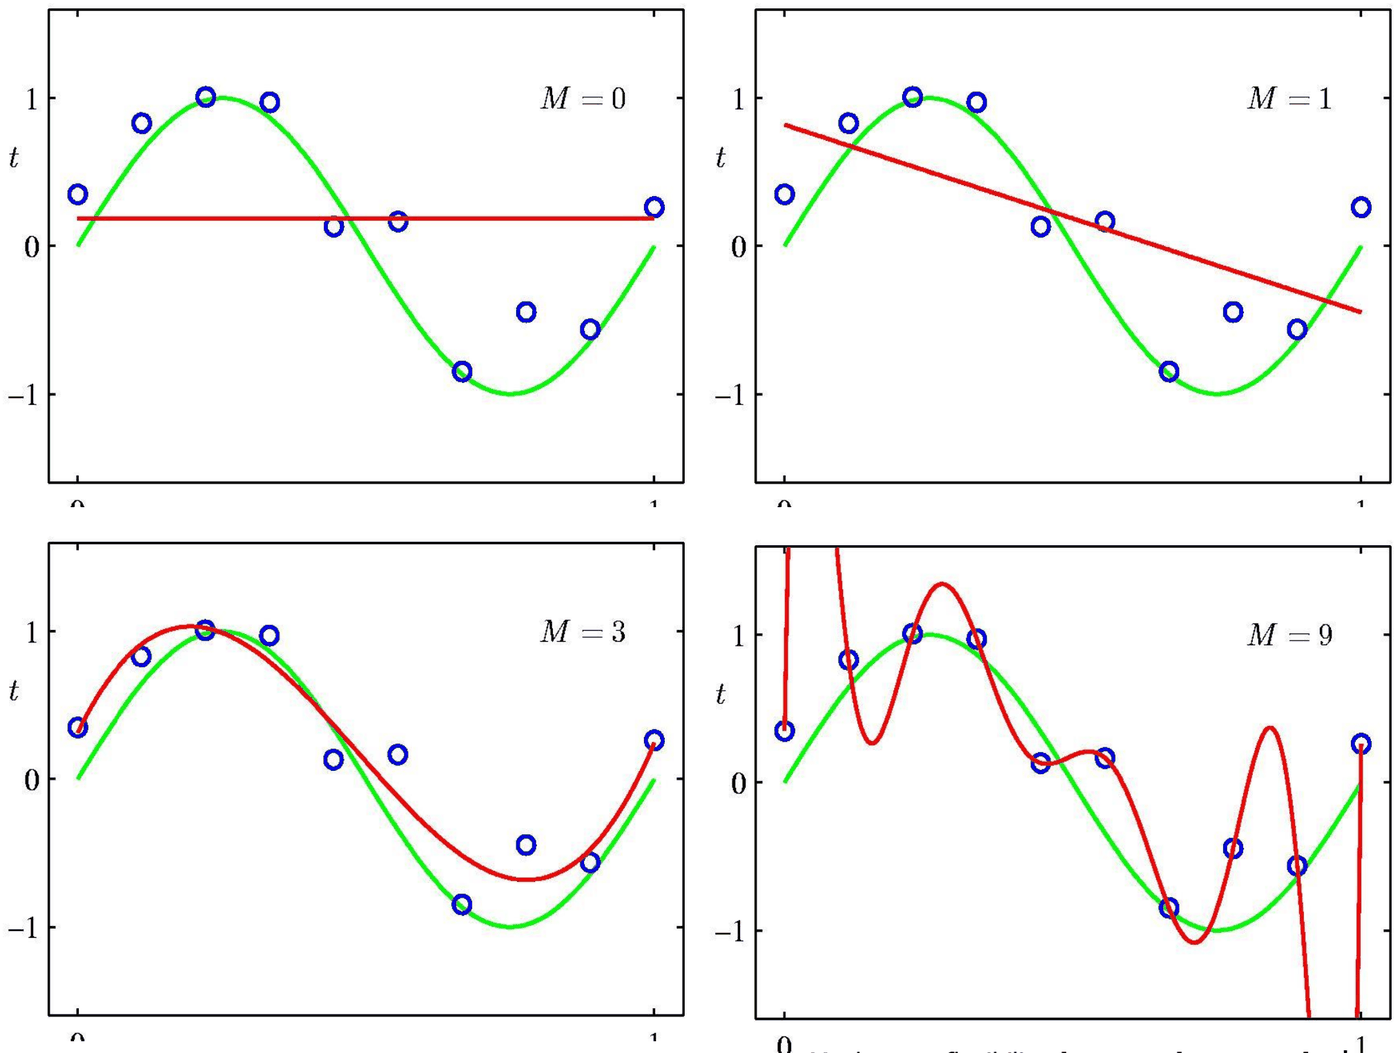
\includegraphics[width=0.91\linewidth,height=0.42\textheight,keepaspectratio]{images/04-l4_polinomi.png}
\caption{Fitting with polynomials of degree \(M = 0, 1, 3, 9\) (in red)
compared to the true function (in green).}
\end{figure}

\begin{itemize}
\tightlist
\item
  \textbf{\(M = 0\)} (constant) and \textbf{\(M = 1\)} (line): the
  model is \textbf{too simple} with respect to the target function and
  fails to capture its trend. This is \textbf{underfitting}.
\item
  \textbf{\(M = 3\)}: more flexibility is useful, and the curve
  approximates the sine well.
\item
  \textbf{\(M = 9\)}: with 10 points and 10 parameters the polynomial
  passes \textbf{exactly} through all data: \(E(\mathbf{w}) = 0\) on the
  training set! But the curve oscillates wildly between the points and
  represents the true function very poorly: the model is too complex
  and \textbf{also learns the noise}. This is \textbf{overfitting}. And
  what about the error on the test set?
\end{itemize}

\subsection{\texorpdfstring{Training and test error as
\(M\) varies}{Training and test error as M varies}}\label{errore-di-training-e-di-test-al-variare-di-m}

To compare models the \textbf{Root-Mean-Square error} is used,
\(E_{RMS} = \sqrt{2E(\mathbf{w}^*)/l}\), where \(E(\mathbf{w}^*)\) is
the error of the trained model. Dividing by \(l\) allows comparing
datasets of different sizes, and the square root brings the error back
to the same scale as the target.

\begin{figure}[htbp]
\centering
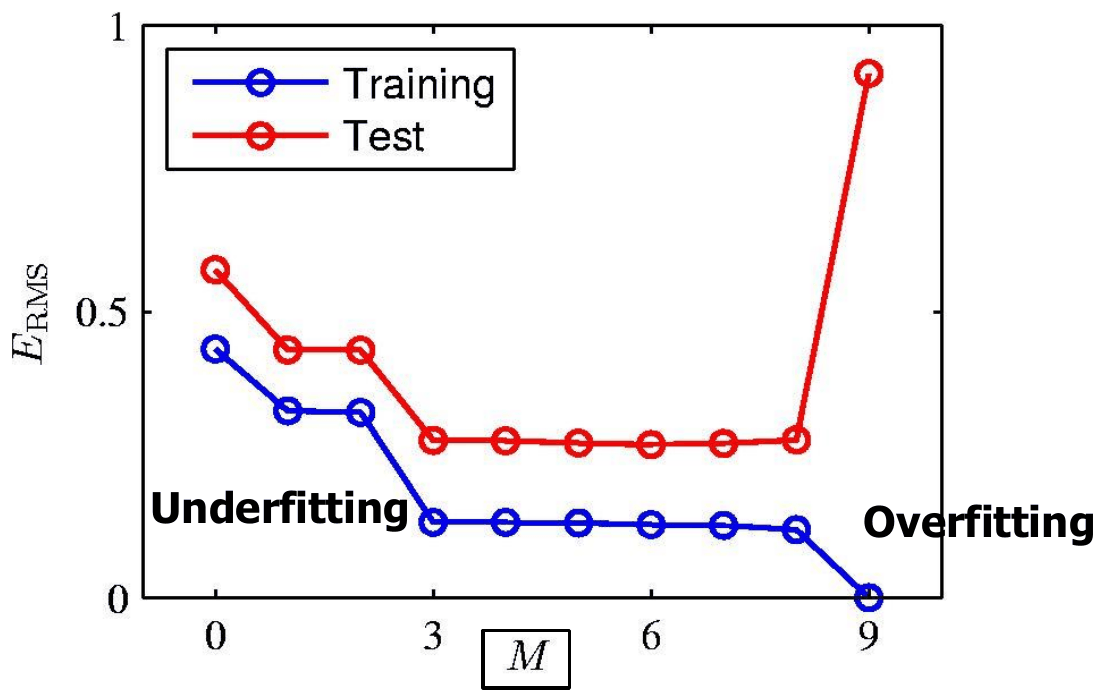
\includegraphics[width=0.60\linewidth,height=0.42\textheight,keepaspectratio]{images/04-l4_rms-vs-M.png}
\caption{Training and test RMS error as the degree \(M\) varies:
underfitting zone on the left, overfitting zone on the right.}
\end{figure}

The training error \textbf{always decreases} as \(M\) increases,
because a more flexible model can fit the data better. The test error
instead first decreases, then stays stable and finally
\textbf{explodes} for \(M = 9\): this is the signature of overfitting.

The optimal \textbf{coefficients} \(\mathbf{w}^*\) are also revealing:

{\def\LTcaptype{none} % do not increment counter
\begin{longtable}[]{@{}lllll@{}}
\toprule\noalign{}
& \(M=0\) & \(M=1\) & \(M=3\) & \(M=9\) \\
\midrule\noalign{}
\endhead
\bottomrule\noalign{}
\endlastfoot
\(w_0^*\) & 0.19 & 0.82 & 0.31 & 0.35 \\
\(w_1^*\) & & −1.27 & 7.99 & 232.37 \\
\(w_2^*\) & & & −25.43 & −5321.83 \\
\(w_3^*\) & & & 17.37 & 48568.31 \\
\(w_4^*\) & & & & −231639.30 \\
\(w_5^*\) & & & & 640042.26 \\
\(w_6^*\) & & & & −1061800.52 \\
\(w_7^*\) & & & & 1042400.18 \\
\(w_8^*\) & & & & −557682.99 \\
\(w_9^*\) & & & & 125201.43 \\
\end{longtable}
}

\begin{boxtip}{Huge weights = overfitting}

In the degree-9 polynomial the coefficients become \textbf{huge} and of
alternating sign: they compensate each other to make the curve pass
exactly through every point, producing very strong oscillations. This
observation is the basis of \textbf{regularisation} (which we will see
with linear models and neural networks): penalising large weights is a
way to control complexity.

\end{boxtip}

\subsection{Effect of the amount of
data}\label{effetto-della-quantituxe0-di-dati}

What happens if, with the same model (\(M = 9\)), we increase the
data?

\begin{figure}[htbp]
\centering
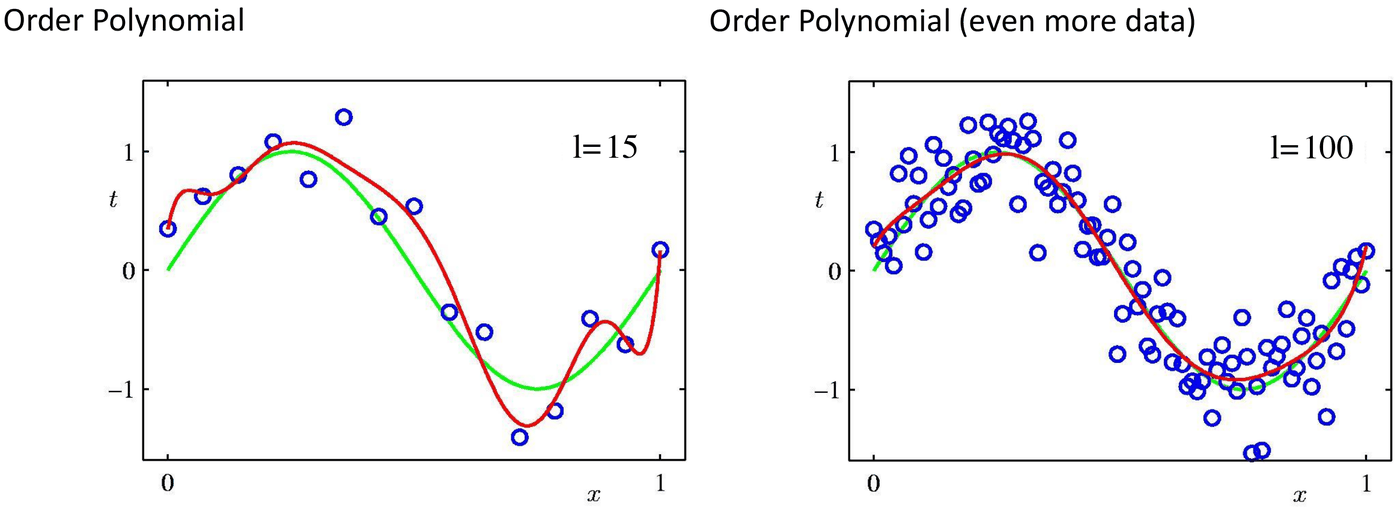
\includegraphics[width=0.91\linewidth,height=0.42\textheight,keepaspectratio]{images/04-l4_polinomio9-dati.png}
\caption{Degree-9 polynomial with \(l = 15\) and \(l = 100\) examples:
with more data overfitting is reduced.}
\end{figure}

With 15 examples the degree-9 polynomial still oscillates, but much
less; with 100 examples it follows the sine almost perfectly.
\textbf{With more data, more complex models can be used} without
falling into overfitting.

\begin{boxabstract}{What we have learned}

Generalisation capability (measured as risk or test error) must be
studied in relation to: - the \textbf{training error} and the
underfitting and overfitting zones; - the \textbf{model complexity}; -
the \textbf{amount of data}.

\textbf{Statistical Learning Theory} is the general theory linking
these three elements.

\end{boxabstract}

\section{Towards Statistical Learning
Theory}\label{verso-la-statistical-learning-theory}

\subsection{The formal setting
(simplified)}\label{il-setting-formale-semplificato}

We want to approximate an unknown function \(f(\mathbf{x})\), where the
target is \(d = f(\mathbf{x}) + \text{noise}\).

Ideally we would like to minimise the \textbf{risk function} (true
error), computed over \textbf{all} possible data: \[
R = \int L\big(d, h(\mathbf{x})\big)\, dP(\mathbf{x}, d),
\] where \(P(\mathbf{x}, d)\) is the (unknown) probability distribution
of the data and \(L\) is a loss, for example
\(L(h(\mathbf{x}), d) = (d - h(\mathbf{x}))^2\). We therefore look for
\(h \in H\) minimising \(R\).

But we only have a finite dataset
\(TR = \{(\mathbf{x}_p, d_p)\}_{p=1}^{l}\). So we minimise the
\textbf{empirical risk} (training error), finding the best values of
the free parameters: \[
R_{emp}(h, TR) = \frac{1}{l} \sum_{p=1}^{l} \big(d_p - h(\mathbf{x}_p)\big)^2.
\] This is the inductive principle of \textbf{Empirical Risk
Minimization} (ERM). The crucial question is: \textbf{can we use
\(R_{emp}\) to approximate \(R\)?}

\begin{figure}[htbp]
\centering
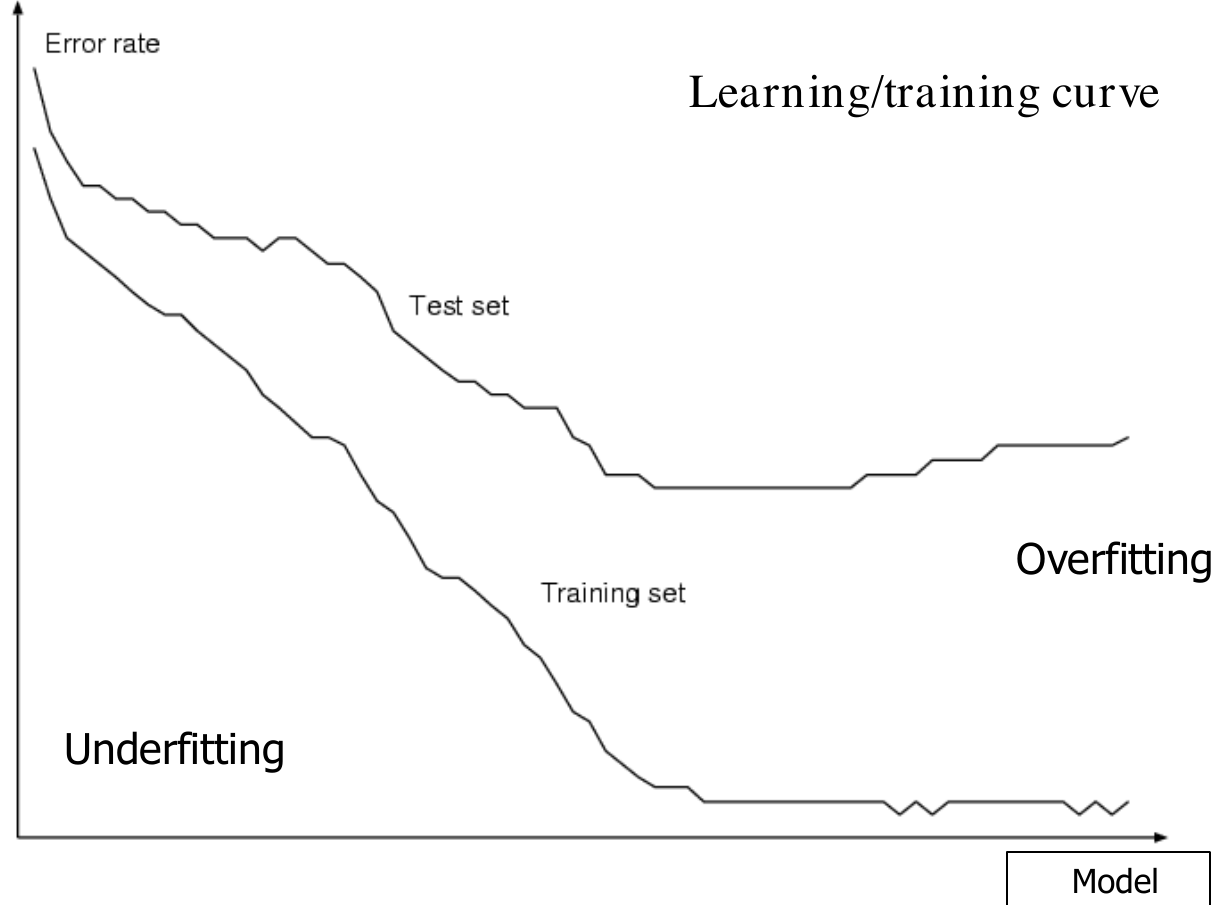
\includegraphics[width=0.57\linewidth,height=0.42\textheight,keepaspectratio]{images/04-l4_curva-apprendimento.png}
\caption{Typical learning behaviour as model complexity grows.}
\end{figure}

\subsection{VC-dimension and risk
bound}\label{vc-dimension-e-bound-sul-rischio}

The \textbf{VC-dimension} (Vapnik-Chervonenkis) is a measure of the
\textbf{complexity} of \(H\), i.e.\ of its flexibility in fitting the
data (for linear models or polynomials it is related to the number of
parameters; it will be formally defined later).

\begin{boxtheorem}{VC-bound}

With probability \(1 - \delta\) it holds: \[
\underbrace{R}_{\text{guaranteed risk}} \;\le\; R_{emp} + \underbrace{\varepsilon\left(\frac{1}{l}, VC, \frac{1}{\delta}\right)}_{\text{VC-confidence}}
\] where the \textbf{VC-confidence} \(\varepsilon\) is a function that
\textbf{grows with the VC-dimension} and \textbf{decreases with the
number of data \(l\)} (and with \(\delta\)).

\end{boxtheorem}

The parameter \(\delta\) is the \textbf{confidence}: it controls the
probability that the bound holds (for example \(\delta = 0.01\) means
that the bound holds with probability \(0.99\)).

This bound \textbf{explains} underfitting and overfitting:

\begin{itemize}
\tightlist
\item
  \textbf{more data} (high \(l\)) → lower VC-confidence, and the bound
  gets closer to \(R\): the empirical risk becomes a good estimate of
  the true one;
\item
  \textbf{model too simple} (low VC-dim) → small \(\varepsilon\), but
  high \(R_{emp}\): \textbf{underfitting};
\item
  \textbf{model too complex} (high VC-dim, fixed \(l\)) → low
  \(R_{emp}\), but \(\varepsilon\) grows, and with it the bound on
  \(R\): \textbf{overfitting}.
\end{itemize}

\begin{figure}[htbp]
\centering
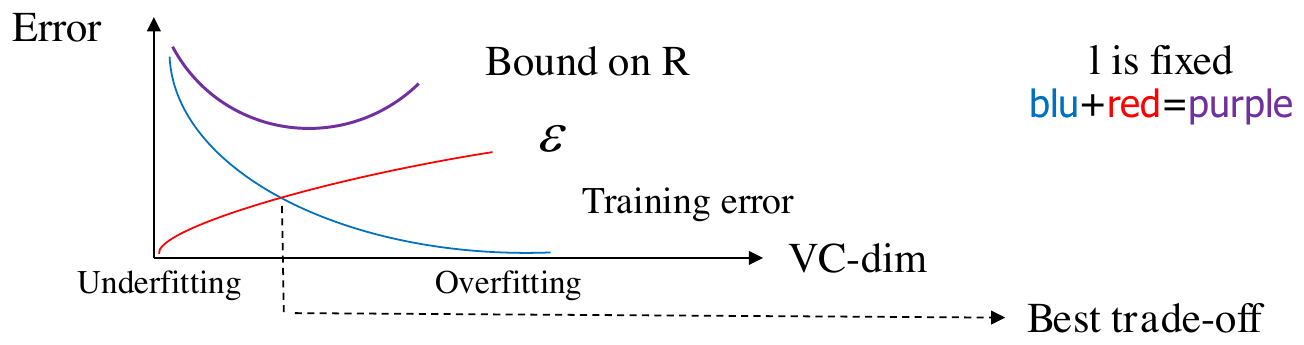
\includegraphics[width=0.80\linewidth,height=0.42\textheight,keepaspectratio]{images/04-l4_bound-vc.png}
\caption{Structural Risk Minimization: the bound on \(R\) (purple) is the
sum of the training error (blue) and the VC-confidence (red); its
minimum is the best trade-off.}
\end{figure}

\begin{boxdefinition}{Structural Risk Minimization (SRM)}

Instead of minimising only \(R_{emp}\), we \textbf{minimise the bound},
i.e.\ the sum of training error and VC-confidence. This formalises the
concept of \textbf{model complexity control}: a trade-off between
complexity (VC-dim) and accuracy on the training set (fitting).

\end{boxdefinition}

A concrete example of a bound is \[
R \le R_{emp} + \varepsilon\left(\frac{VC}{l}, -\frac{\ln\delta}{l}\right),
\] and there are various formulations for different function classes
and tasks. In simple words: \textbf{\(f\) can be approximated well from
examples provided that we have a good number of data and the model
complexity is suited to the problem}. One must fit the data as much as
possible to avoid underfitting (high \(R_{emp}\)), but not too much, to
avoid overfitting (due to the growth of the VC-confidence).

\begin{boxnote}{Beyond the classical trade-off}

More recent phenomena such as \textbf{double descent},
over-parameterisation and \emph{benign overfitting} (typical of deep
networks) seem to challenge this view and will be discussed later in
the course.

\end{boxnote}

\subsection{Why SLT is
important}\label{perchuxe9-la-slt-uxe8-importante}

SLT makes it possible to frame formally the problem of generalisation
and overfitting, providing \textbf{analytical upper bounds} on the risk
\(R\) regardless of the type of algorithm or the details of the model.
It shows that ML is \textbf{well founded}: the risk can be bounded
analytically, and few concepts are fundamental. It has also led to new
models (\textbf{SVMs}) that directly take complexity control into
account, and it explains the main difference between ML and pure
optimisation methods (which provide the techniques for
\emph{fitting}): in ML the goal is not to minimise the error on the
data, but on \emph{future} data.

Practical questions remain open: how to measure complexity? How to find
the best trade-off between fitting and complexity?

\begin{boxquestion}{Exercises proposed by the professor}

\begin{itemize}
\tightlist
\item
  Why does a zero training error not necessarily imply a good
  solution?
\item
  Relate underfitting and overfitting to the interpretation of the SLT
  inequality and to the polynomial example.
\item
  Looking at the definition of overfitting, identify \(h\) and \(h'\)
  on the SLT bound plot. \emph{(Hint: \(h\) is to the right of the
  minimum, with lower \(R_{emp}\) but higher bound; \(h'\) is near the
  minimum.)}
\item
  Is noise the cause of overfitting, or is it the complexity
  trade-off? Can overfitting occur even with perfectly clean data?
  \emph{(Yes: even without noise, a very high-degree polynomial
  interpolating a few points of a smooth function can oscillate a lot
  between one point and the next; the problem is excessive complexity
  relative to the available data.)}
\end{itemize}

\end{boxquestion}

\section{Validation}\label{validazione}

Evaluating the performance of an ML system means evaluating its
\textbf{predictive accuracy}. Beware: \textbf{performance on the
training data gives an overly optimistic evaluation}. Hence the mantra
``validation, validation, validation''. Here we give an introduction;
validation will be taken up again in dedicated lectures.

\subsection{The two goals of
validation}\label{i-due-obiettivi-della-validazione}

\begin{boxdefinition}{Model selection and model assessment}

\begin{itemize}
\tightlist
\item
  \textbf{Model selection}: estimate the performance (generalisation
  error) of \textbf{different models} in order to choose the best one.
  It includes searching for the best \textbf{hyperparameters}
  (e.g.\ the degree of the polynomial). \emph{Returns a model.}
\item
  \textbf{Model assessment}: having chosen the final model, estimate
  its prediction error (risk) on \textbf{new test data}, as a measure
  of the quality of the chosen model. \emph{Returns an estimate.}
\end{itemize}

\end{boxdefinition}

\begin{boxwarning}{Golden rule}

Keep the \textbf{goals separate} and use \textbf{separate data sets}
for each. If the test set is used to choose the model, the final
estimate is no longer reliable (it is optimistic).

\end{boxwarning}

In an ideal world we would have a large training set (to find the best
hypothesis), a large validation set for model selection and a very
large external test set. With finite, often small, datasets, we can
only \textbf{estimate} generalisation.

\subsection{Hold-out}\label{hold-out}

In the basic technique, \textbf{hold-out}, the dataset \(D\) is
partitioned into three \textbf{disjoint} sets:

\begin{itemize}
\tightlist
\item
  \textbf{Training set (TR)}: used to run the learning algorithm;
\item
  \textbf{Validation set (VL)} or \emph{selection set}: used to choose
  the best model (e.g.\ hyperparameter tuning);
\item
  \textbf{Test set (TS)}: used \textbf{only} for model assessment,
  never to choose or tune \(h\).
\end{itemize}

TR and VL together form the \textbf{development/design set}; the test
set (for example 25--30\% of the data) is kept aside.

\begin{figure}[htbp]
\centering
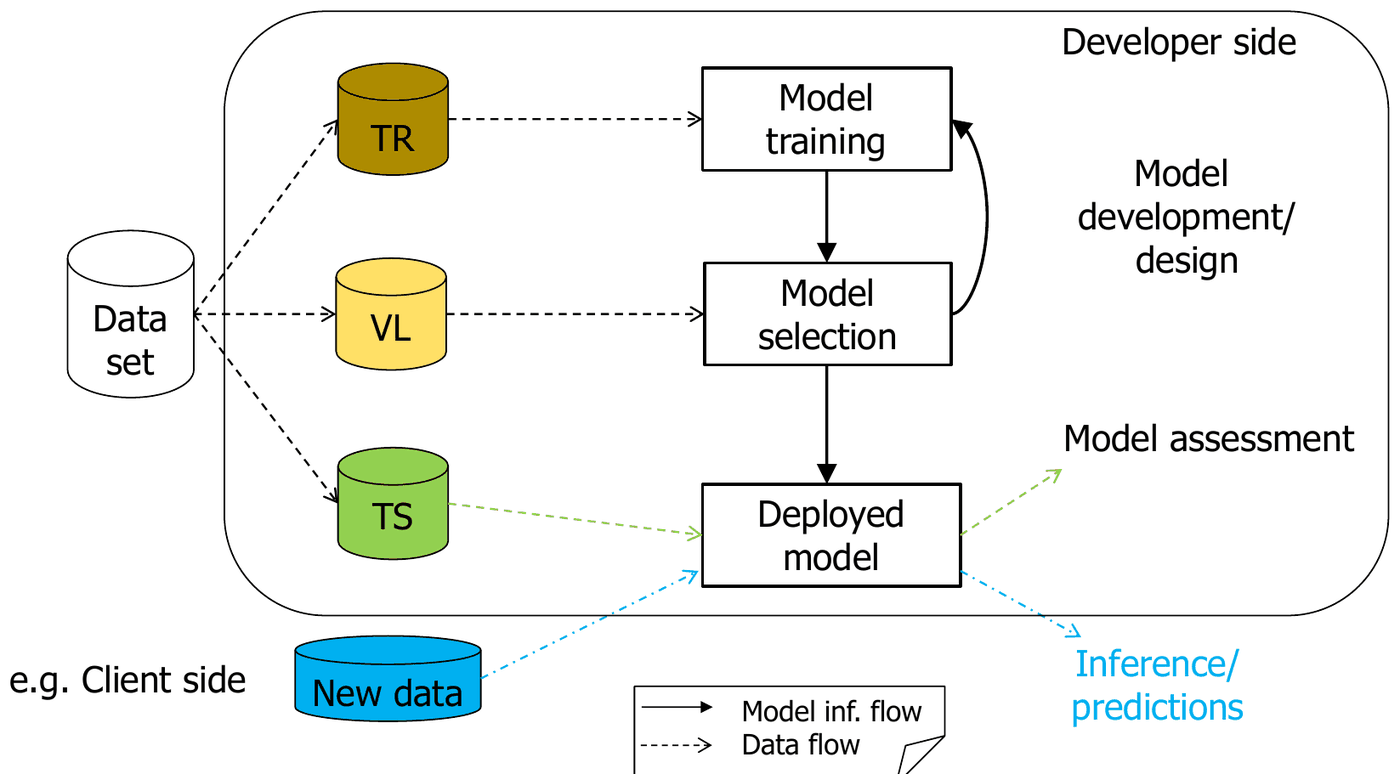
\includegraphics[width=0.86\linewidth,height=0.42\textheight,keepaspectratio]{images/04-l4_schema-tr-vl-ts.png}
\caption{Role of TR, VL and TS: model development on the developer side,
use in inference on the client side.}
\end{figure}

\subsection{K-fold cross-validation
(preview)}\label{k-fold-cross-validation-anticipazione}

Hold-out can make poor use of the data, especially when they are few.
In \textbf{K-fold cross-validation}:

\begin{enumerate}
\def\labelenumi{\arabic{enumi}.}
\tightlist
\item
  \(D\) is split into \(k\) mutually exclusive subsets
  \(D_1, \dots, D_k\);
\item
  for each \(i\), train on \(D \setminus D_i\) and evaluate on
  \(D_i\);
\item
  the \(k\) results are combined.
\end{enumerate}

\begin{figure}[htbp]
\centering
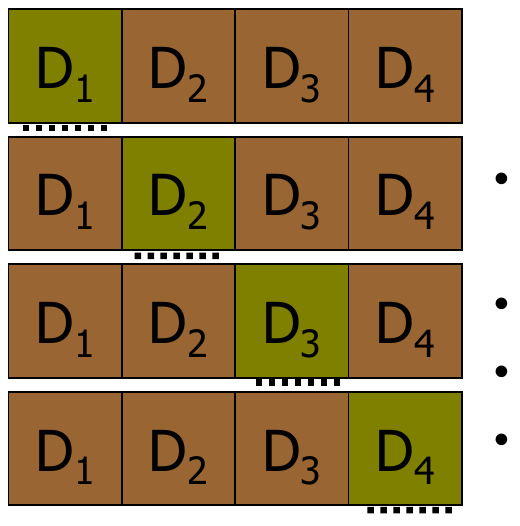
\includegraphics[width=0.29\linewidth,height=0.42\textheight,keepaspectratio]{images/04-l4_kfold.png}
\caption{4-fold cross-validation: each fold in turn acts as the
validation set.}
\end{figure}

In this way all data are used both for training and for validation (or
testing). It can be applied both to the validation split and to the
test split. Open questions are how many folds to use (3, 5, 10, up to
\emph{leave-one-out}), the often high computational cost and the
combination with other schemes (validation set, double K-fold). It will
be discussed in detail later.

\section{Accuracy in
classification}\label{accuratezza-nella-classificazione}

\subsection{Confusion matrix}\label{matrice-di-confusione}

For a binary classifier, the actual class and the predicted class are
compared:

{\def\LTcaptype{none} % do not increment counter
\begin{longtable}[]{@{}lll@{}}
\toprule\noalign{}
Actual ~Predicted & Positive & Negative \\
\midrule\noalign{}
\endhead
\bottomrule\noalign{}
\endlastfoot
\textbf{Positive} & TP (true positives) & FN (false negatives) \\
\textbf{Negative} & FP (false positives) & TN (true negatives) \\
\end{longtable}
}

From which:

\begin{itemize}
\tightlist
\item
  \textbf{Accuracy} \(= \dfrac{TP + TN}{\text{total}}\): percentage of
  correctly classified patterns;
\item
  \textbf{Sensitivity} (\emph{True Positive rate}, \emph{Recall})
  \(= \dfrac{TP}{TP + FN}\): how many actual positives are recognised;
\item
  \textbf{Specificity} (\emph{True Negative rate})
  \(= \dfrac{TN}{FP + TN} = 1 - FPR\): how many actual negatives are
  recognised;
\item
  \textbf{Precision} \(= \dfrac{TP}{TP + FP}\): how many of the
  predicted positives are actually positive.
\end{itemize}

A false positive is equivalent to a \textbf{false alarm}.

\begin{boxwarning}{Beware of accuracy}

\begin{itemize}
\tightlist
\item
  For binary classification, 50\% accuracy is that of a
  \textbf{random} predictor (coin toss).
\item
  With \textbf{unbalanced data} (e.g.\ 99\% positives) there is a
  trivial classifier that always answers ``positive'' and has 99\%
  accuracy without having learned anything. In these cases accuracy
  alone is misleading.
\end{itemize}

\end{boxwarning}

\subsection{ROC curve}\label{curva-roc}

The \textbf{ROC curve} shows the \emph{True Positive rate}
(sensitivity) as a function of the \emph{False Positive rate}
(\(1 -\) specificity) as the decision threshold of the classifier
varies.

\begin{figure}[htbp]
\centering
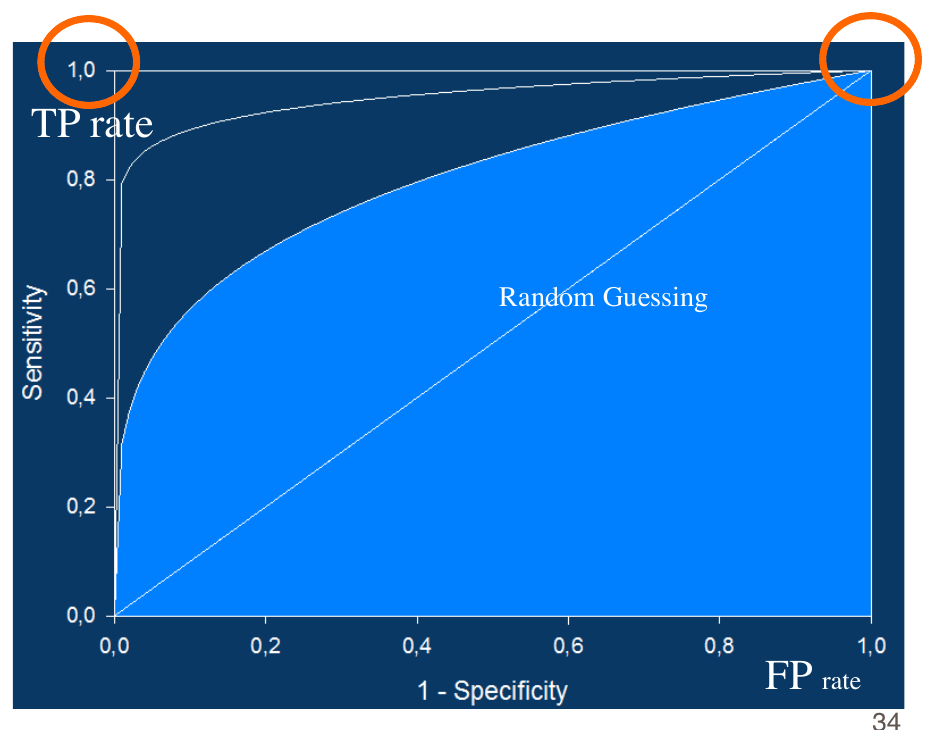
\includegraphics[width=0.49\linewidth,height=0.42\textheight,keepaspectratio]{images/04-l4_roc.png}
\caption{ROC curve: the diagonal corresponds to the random classifier;
better curves have a larger area under the curve (AUC).}
\end{figure}

The \textbf{diagonal} corresponds to the worst (random) classifier.
Better curves rise quickly towards the top-left corner (high TPR with
low FPR) and have a higher \textbf{AUC} (\emph{Area Under the Curve}):
the ideal classifier has AUC \(= 1\), the random one \(0.5\).

\section{The design cycle}\label{il-ciclo-di-progettazione}

\begin{figure}[htbp]
\centering
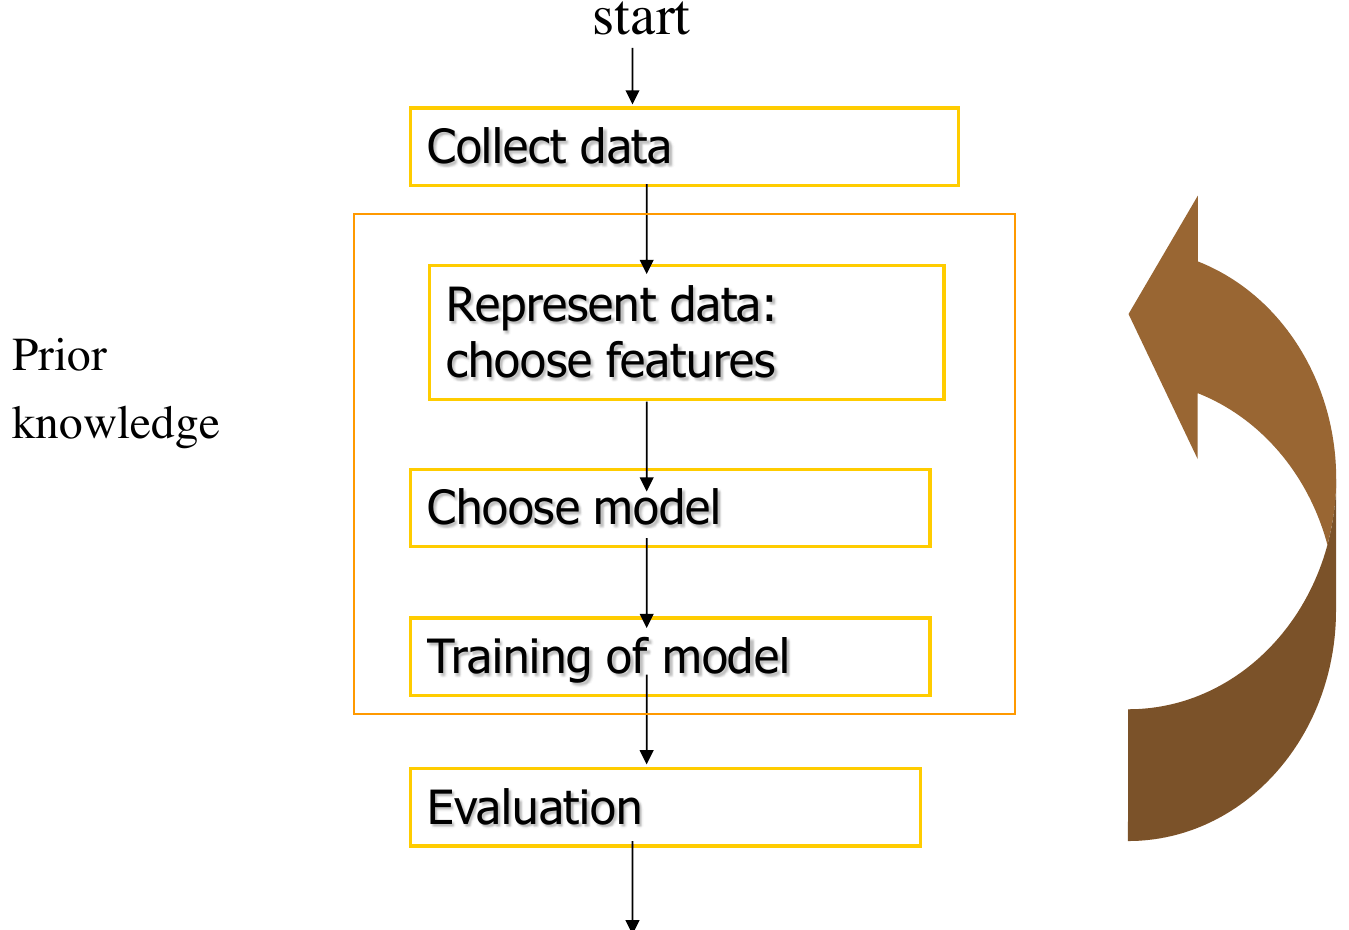
\includegraphics[width=0.57\linewidth,height=0.42\textheight,keepaspectratio]{images/04-l4_ciclo-progettazione.png}
\caption{The design cycle of an ML system: an iterative process guided by
prior knowledge.}
\end{figure}

\begin{enumerate}
\def\labelenumi{\arabic{enumi}.}
\tightlist
\item
  \textbf{Data collection}: selection, integration, cleaning. A
  \textbf{large and representative} enough set of examples is needed
  for training and testing.
\item
  \textbf{Data representation}: depends on the domain and exploits the
  expert's prior knowledge; includes feature selection, outlier
  detection, variable scaling, handling of missing data. \textbf{It is
  often the most critical phase} for overall success.
\item
  \textbf{Model choice}: formulation of the problem and of the
  hypotheses. One must know the model's \textbf{limits of
  applicability} and control its complexity.
\item
  \textbf{Model building} (the heart of ML): through the learning
  algorithm on the training data.
\item
  \textbf{Evaluation}: performance is \textbf{predictive accuracy};
  interpretation of results, explanation of data and knowledge
  extraction are added.
\item
  \textbf{Deployment}.
\end{enumerate}

The cycle is iterative: the results of the evaluation may require going
back to previous phases.

\section{Interpretation errors}\label{errori-di-interpretazione}

For every statistical model (including Data Mining and ML):

\begin{itemize}
\tightlist
\item
  \textbf{causality} is (often) assumed and a data set
  \textbf{representative} of the phenomenon is needed. ML does not work
  with uncorrelated variables or random phenomena (lotteries);
  uninformative inputs lead to poor models and results;
\item
  \textbf{causality cannot be inferred from data analysis alone}: in
  Florida people are on average older than in the other US states, but
  it is not the climate that makes them live longer (people move there
  when retired). Statistical dependence can have reasons external to
  the data.
\end{itemize}

Specific to ML: \textbf{powerful models increase the risk}, because
they also fit ``garbage'' data; and results that are \textbf{not
properly validated} may lead to misleading predictions and
interpretations.

\begin{boxabstract}{Summary}

Generalisation depends on the trade-off between \textbf{model
complexity} and \textbf{amount of data}. Models that are too simple
\textbf{underfit}, models that are too complex \textbf{overfit} (low
training error, high test error). SLT formalises everything with the
\textbf{VC-bound} \(R \le R_{emp} + \varepsilon(1/l, VC, 1/\delta)\)
and suggests \textbf{Structural Risk Minimization}. In practice
generalisation is estimated through \textbf{validation}: \emph{model
selection} (on VL) and \emph{model assessment} (on TS), always on
separate data.

\end{boxabstract}

\begin{boxquestion}{Possible exam questions}

\begin{itemize}
\tightlist
\item
  Formally define overfitting.
\item
  Describe the polynomial fitting example: what happens as \(M\) and
  \(l\) vary?
\item
  Write the VC-bound and explain how it justifies underfitting and
  overfitting.
\item
  Difference between risk \(R\) and empirical risk \(R_{emp}\); what
  is the ERM principle?
\item
  Difference between model selection and model assessment; why are
  separate sets needed?
\item
  Define accuracy, sensitivity, specificity, precision; what is the ROC
  curve?
\end{itemize}

\end{boxquestion}
